\chapter{Methodology}
\label{chap:methodology}

\section{Abbreviations}

You can define abbreviations and refer to them like this: The \gls{dsr} methodology is widely used in information systems research. The \gls{dsr} approach emphasizes the creation and evaluation of artifacts to solve identified problems.

\section{Figures}

\begin{figure}[htbp!]
    \centering
    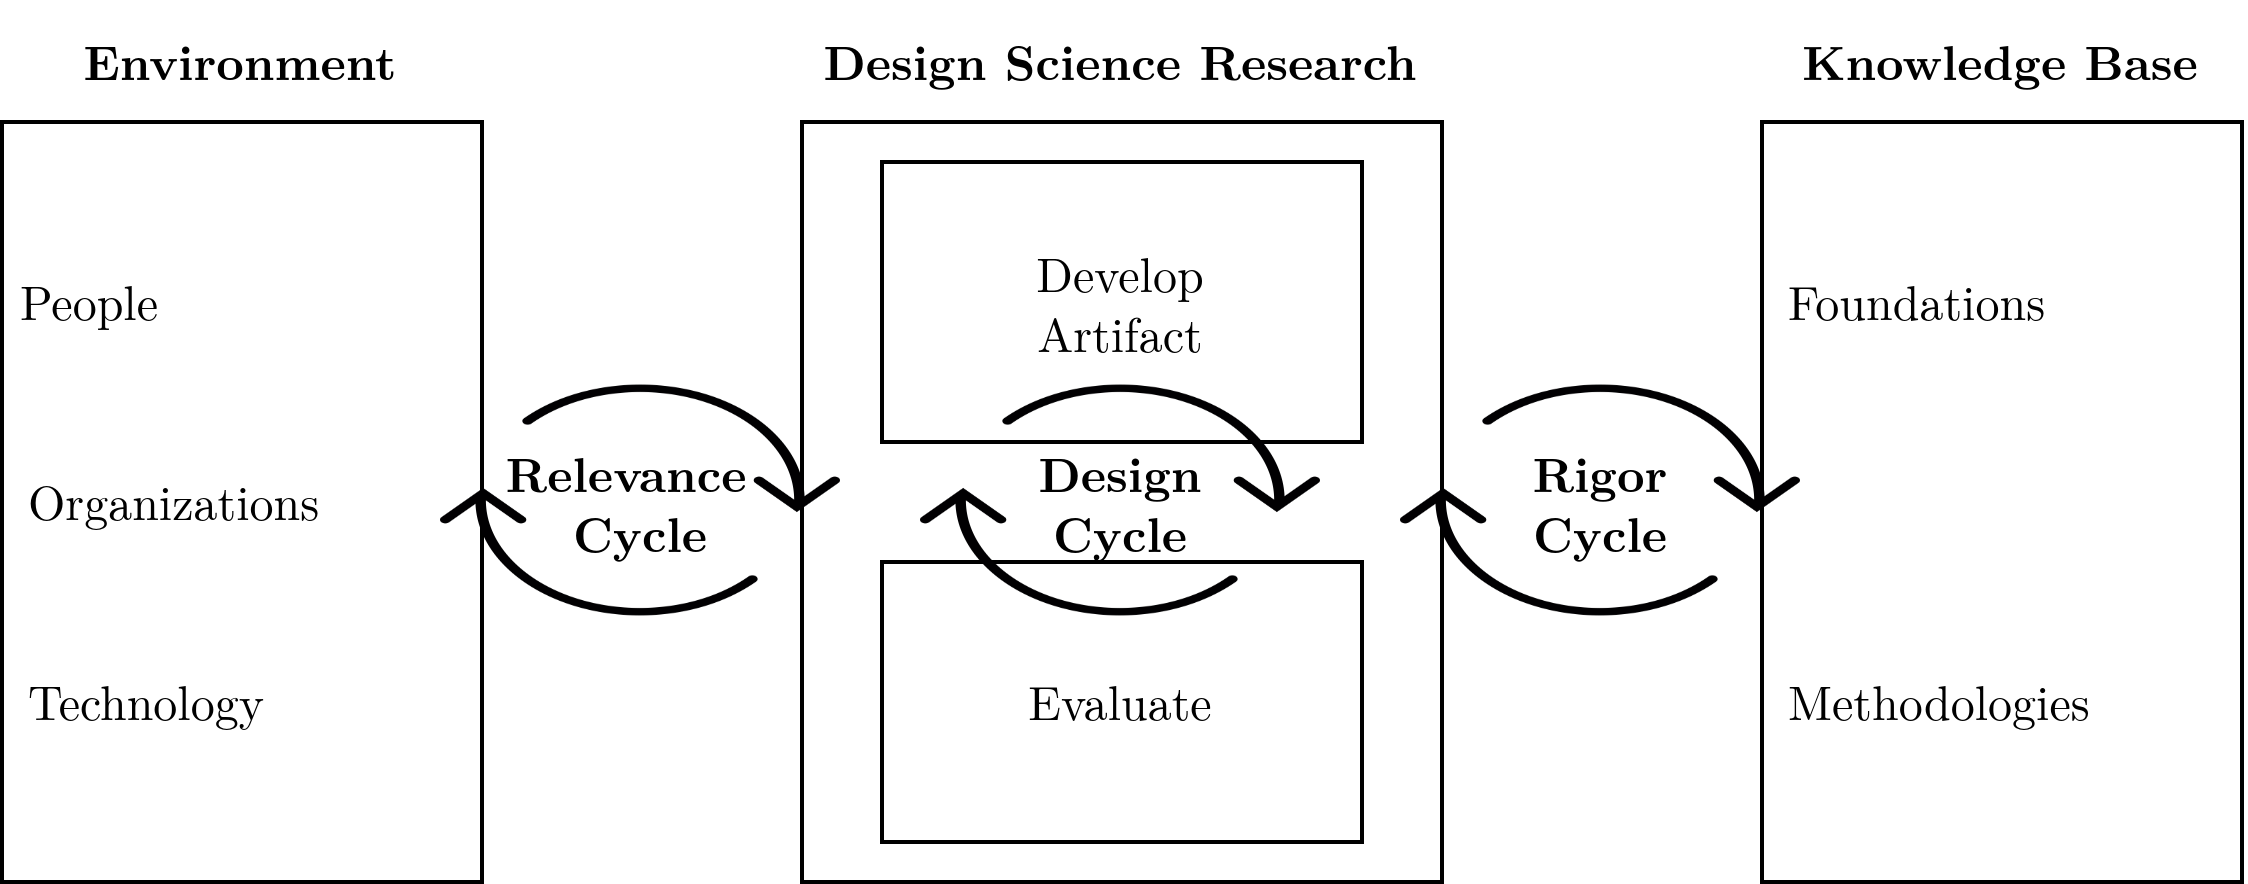
\includegraphics[width=0.9\textwidth]{figures/design-science-generic.png}
    \caption[DSR approach with relevance, rigor, and design cycle.]{DSR approach with relevance, rigor, and design cycle. Adapted from~\textcite{hevner2004design}.}
    \label{fig:design-science-generic}
\end{figure}

You can include figures and refer to them like this: Figure~\ref{fig:design-science-generic} shows the \gls{dsr} approach with relevance, rigor, and design cycle.
